\documentclass[11pt]{article}

\usepackage[margin=1in]{geometry}
\usepackage{amsmath,amssymb,amsthm}
\usepackage{graphicx}
\usepackage[hidelinks]{hyperref}

\newtheorem{theorem}{Theorem}
\newtheorem{lemma}{Lemma}
\newtheorem{corollary}{Corollary}

\newcommand{\N}{\mathbb{N}}
\newcommand{\SB}{\mathrm{SB}}
\newcommand{\SD}{\mathrm{SD}}
\newcommand{\cB}{\mathcal{B}}
\newcommand{\cD}{\mathcal{D}}
\newcommand{\cW}{\mathcal{W}}
\newcommand{\REFL}{\mathrm{REFL}}

\title{Borel measurable factor-subspace selection in parametrized weakly compact factorization}
\author{arXiv automatic math run \texttt{fa\_banach\_001}}
\date{June 14, 2026}

\begin{document}
\maketitle

\section*{Source Question}

This packet addresses Question 6.1 of Antunes--Beanland--Braga,
\emph{Uniformly Factoring Weakly Compact operators and Parametrized Dualization},
arXiv:1909.07475 \cite{AntunesBeanlandBraga}. The question appears on PDF page 30.

\begin{center}
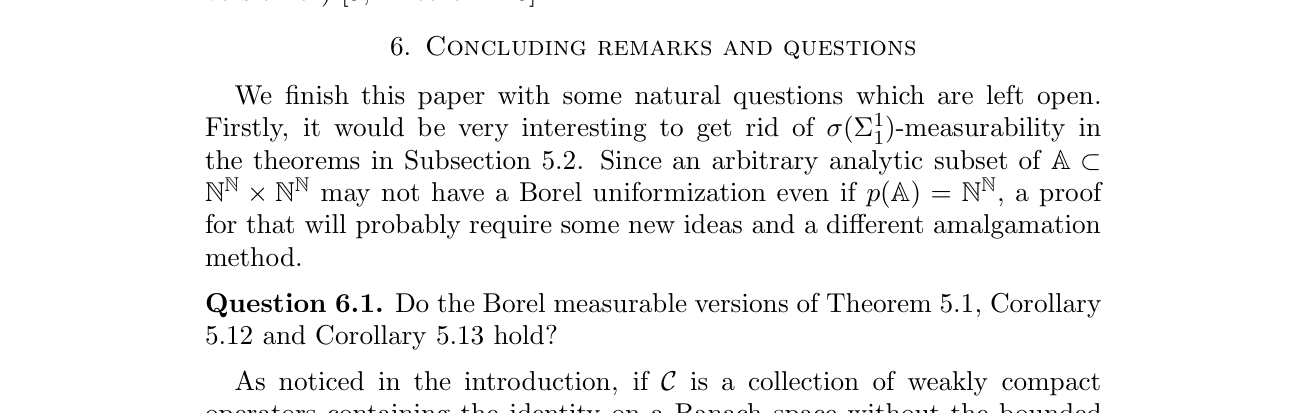
\includegraphics[width=\textwidth]{figures/open_question_page30.png}
\end{center}

The question asks whether the Borel measurable versions of Theorem 5.1,
Corollary 5.12, and Corollary 5.13 of the source paper hold. The answer is yes.

\section*{Proof Intuition}

The proof of Theorem 5.1 in \cite{AntunesBeanlandBraga} already constructs
Borel maps up to the final rational-amalgamation step. At that point the paper
has a Borel code map
\[
   \eta=\psi\circ\sigma:\cB\to\N^\N
\]
whose range is analytic. The published proof chooses an arbitrary closed tree
whose projection is this analytic range and then invokes Jankov--von Neumann
uniformization, obtaining only $\sigma(\Sigma^1_1)$-measurability.

The key observation is that this arbitrary tree is unnecessary. Since the
analytic set in question is specifically the image of a Borel map, one can
build the closed tree from a closed parametrization of the Borel graph of
$\eta$. This gives a Borel branch selector for the actual parameter $A\in\cB$.
Every branch of the new tree still has first coordinate $\eta(A_0)$ for some
original $A_0\in\cB$, so the reflexivity argument in the Kurka amalgamation
step is unchanged.

\section*{A closed-tree lift for Borel images}

\begin{lemma}\label{lem:closed-lift}
Let $S$ be a standard Borel space and let $\eta:S\to\N^\N$ be Borel. Then
there are a closed set $C\subset\N^\N\times\N^\N$ and a Borel map
\[
   \tau:S\to C
\]
such that, writing $p$ for projection onto the first coordinate,
\[
   p(C)=\eta(S)
   \quad\text{and}\quad
   p(\tau(s))=\eta(s)\quad(s\in S).
\]
Moreover every branch $(\alpha,\gamma)\in C$ has $\alpha=\eta(s)$ for some
$s\in S$.
\end{lemma}

\begin{proof}
Choose a Borel isomorphism $i:S\to S_0$, where $S_0$ is a Borel subset of
$\N^\N$. The map
\[
   s\mapsto (i(s),\eta(s))
\]
is Borel and injective, so its image
\[
   G=\{(i(s),\eta(s)):s\in S\}\subset\N^\N\times\N^\N
\]
is Borel by the Lusin--Souslin theorem.

Use the standard representation theorem that every Borel subset of a Polish
space is a one-to-one continuous image of a closed subset of Baire space
\cite[Theorem 13.7]{Kechris}. Thus there are a closed set
$P\subset\N^\N$ and a continuous bijection
\[
   h:P\to G.
\]
Write $h(z)=(h_1(z),h_2(z))$. Define
\[
   C=\{(h_2(z),z):z\in P\}.
\]
Since $P$ is closed and $h_2$ is continuous, $C$ is closed. Also
$p(C)=h_2(P)=\eta(S)$.

The inverse $h^{-1}:G\to P$ is Borel, again by Lusin--Souslin. Hence
\[
   \tau(s)=\bigl(\eta(s),h^{-1}(i(s),\eta(s))\bigr)
\]
is a Borel map from $S$ into $C$, and $p(\tau(s))=\eta(s)$. The final assertion
follows from $p(C)=\eta(S)$.
\end{proof}

\section*{Borel version of Theorem 5.1}

\begin{theorem}\label{thm:borel-factor-subspaces}
Let $\cB\subset \cW_{\SB,\SD}$ be Borel. Then the maps in Theorem 5.1 of
\cite{AntunesBeanlandBraga} may be chosen Borel: there are a reflexive
space $Z\in\SB$, a Borel map $\Psi:\cB\to\SB(Z)$, and a Borel map
\[
   \Phi:\cD\to Z,\qquad
   \cD=\{(X,Y,\widehat A,x)\in\cB\times C(\Delta):x\in X\},
\]
such that for every $A=(X,Y,\widehat A)\in\cB$,
\begin{enumerate}
\item $\Phi_A(X)=\Psi(A)$,
\item $\Phi_A:X\to Z$ is bounded linear with $\|\Phi_A\|\le 1$, and
\item $A=L\circ\Phi_A$ for some bounded operator $L:\Psi(A)\to Y$.
\end{enumerate}
\end{theorem}

\begin{proof}
We use the notation of the proof of Theorem 5.1 in
\cite{AntunesBeanlandBraga}. The preceding factorization-through-a-Borel-basic-sequence
theorem in that paper gives
Borel maps
\[
   \sigma:\cB\to C(\Delta)^\N,\qquad
   \varphi:\cD\to C(\Delta),
\]
where $\sigma(A)$ is a normalized shrinking boundedly complete basic sequence
and $A$ factors through $\overline{\mathrm{span}}\{\sigma(A)\}$ via
$\varphi_A$. Let $\psi:\mathrm{mbs}\to\N^\N$ be the rational-code map from
Lemma 5.10 of the source paper, and set
\[
   \eta(A)=\psi(\sigma(A)).
\]
Then $\eta:\cB\to\N^\N$ is Borel.

Apply Lemma \ref{lem:closed-lift} to $S=\cB$ and this $\eta$. Let
$C\subset\N^\N\times\N^\N$ be the closed set obtained there, and let
$\tau:\cB\to C$ be the Borel lift. Let $T$ be the pruned tree on
$\N\times\N$ with $[T]=C$.

Now repeat the Kurka amalgamation construction from the proof of Theorem 5.1,
using this tree $T$. Namely define the norm on $c_{00}(T)$ by
\[
   \|x\|
   =
   \sup_{\beta\in [T]}
   \left\|
       \sum_{t\prec\beta} x(t) r_{|t|}
   \right\|_{p(\beta)},
\]
let $E$ be the completion, let $E_\beta$ be the branch subspace, set
\[
   W=\overline{\mathrm{conv}}\bigcup_{\beta\in[T]} B_{E_\beta},
   \qquad
   Z=\Delta_2(E,W),
\]
and view $Z$ as an element of $\SB$.

The reflexivity proof is unchanged. Indeed, if $\beta\in[T]=C$, then
$p(\beta)=\eta(A_0)=\psi(\sigma(A_0))$ for some $A_0\in\cB$ by
Lemma \ref{lem:closed-lift}. The source proof shows that
$F_{\psi(\sigma(A_0))}$ is reflexive. Hence every branch space $E_\beta$ is
reflexive, and Kurka's proposition used in the source proof implies that
$Z$ is reflexive.

For $A\in\cB$, put $t_A=\tau(A)$. Since $p(t_A)=\eta(A)$, the same branch
isometry as in the source proof embeds $F_{\eta(A)}$ into $Z$ along the branch
$t_A$. Define
\[
   \Phi(X,Y,\widehat A,x)
      =
      I_A\bigl(U_{\sigma(A)}(\varphi(X,Y,\widehat A,x))\bigr),
\]
and
\[
   \Psi(A)
      =
      \overline{\mathrm{span}}\{\Phi(A,d_n(X)):n\in\N\},
\]
exactly as in \cite{AntunesBeanlandBraga}.

All algebraic and norm estimates are identical to the published proof, so
$\Phi_A(X)=\Psi(A)$, $\|\Phi_A\|\le 1$, and $A$ factors through $\Psi(A)$.
It remains only to note the measurability. In the source proof, the only
non-Borel input is the map $A\mapsto t_A$, obtained there by
Jankov--von Neumann uniformization. Here $A\mapsto t_A=\tau(A)$ is Borel.
The displayed formula in the source proof for preimages of open balls under
$\Phi$ therefore gives Borel, rather than merely
$\sigma(\Sigma^1_1)$, preimages. Consequently $\Phi$ is Borel. Since the
Kuratowski--Ryll-Nardzewski selectors $d_n$ are Borel, the map
$A\mapsto \overline{\{\Phi(A,d_n(X)):n\in\N\}}$ is Borel into $\SB(Z)$.
Thus $\Psi$ is Borel as well.
\end{proof}

\section*{Consequences for the two corollaries}

\begin{corollary}
The Borel measurable versions of Corollary 5.12 and Corollary 5.13 of
\cite{AntunesBeanlandBraga} hold.
\end{corollary}

\begin{proof}
For Corollary 5.12, apply Theorem \ref{thm:borel-factor-subspaces} to the
Borel family of identity operators on the given Borel subset of $\REFL$,
as in the source proof. The isometric-embedding conclusion and the Borel
measurability of the point map follow from the Borel map $\Phi$ above.

For Corollary 5.13, the source paper states that the proof is a mix of
Braga's parametrized Zippin theorem \cite{Braga2015} and Corollary 5.12, and
that the incorrect Borel claim in \cite{Braga2015} comes from the same
rational-amalgamation uniformization step. Before that final step the
assignments are Borel; applying Lemma \ref{lem:closed-lift} to the resulting
Borel rational-code map supplies a Borel branch selector. Repeating the
remaining Kurka amalgamation argument gives a space $Z\in\SD$ with a shrinking
basis and Borel maps $\Psi$ and $\psi$ with the asserted properties.
\end{proof}

\section*{Novelty and verification notes}

Run-index and local parsed-corpus searches for this arXiv id, the named
theorems and corollaries, and the main uniformization phrases found no previous
packet or apparent later answer. Bounded web searches on 2026-06-14 for exact
phrases from Question 6.1, including its theorem/corollary numbering and author
names, found no later answer besides the source arXiv page and the earlier
Braga paper corrected in the source paper.

A deeper citation check found the published version of the source paper as
\emph{Forum of Mathematics, Sigma} 9 (2021), e22, DOI
\texttt{10.1017/fms.2020.68}. Crossref reports no citing works for this DOI,
while OpenAlex reports exactly one citing work: Cuth--Dolezal--Doucha--Kurka,
\emph{Polish spaces of Banach spaces: Complexity of isometry and isomorphism
classes}, DOI \texttt{10.1017/s1474748023000440}. Text extraction from the
published PDF of that citing work shows the source paper only in the
bibliography and gives no hits for the specific open-question vocabulary.
arXiv API exact-phrase searches for the key labels and question phrases also
returned zero results. Semantic Scholar API access was rate-limited during the
audit.

This is a deeper bounded novelty check, not an exhaustive proof of historical
priority.

The main review point is Lemma \ref{lem:closed-lift}: once the closed tree is
chosen from the Borel graph of $\eta$, every downstream step is the published
proof with ``Borel'' substituted for ``$\sigma(\Sigma^1_1)$'' at the single
uniformization bottleneck.

\begin{thebibliography}{9}

\bibitem{AntunesBeanlandBraga}
L. Antunes, K. Beanland, and B. de Mendonca Braga,
\emph{Uniformly Factoring Weakly Compact operators and Parametrized Dualization},
arXiv:1909.07475, 2019.

\bibitem{Braga2015}
B. M. Braga,
\emph{Duality on Banach spaces and a Borel parametrized version of Zippin's theorem},
Ann. Inst. Fourier (Grenoble) 65 (2015), no. 6, 2413--2435.

\bibitem{Kechris}
A. S. Kechris,
\emph{Classical Descriptive Set Theory},
Graduate Texts in Mathematics 156, Springer, 1995.

\bibitem{Kurka}
O. Kurka,
\emph{Amalgamations of classes of Banach spaces with a monotone basis},
Studia Math. 234 (2016), no. 2, 121--148.

\end{thebibliography}

\end{document}
